%%%%%%%%%%%%%%%%%%%%%%%%%%%%%%%%%%%%%%%%%%%%%%%%%%%%%%%%%%%%%%%%%%%%%%%
%
% Generic Methodology for Physical Climate Risk Modelling
%
% 2021 OS-Climate
%
%%%%%%%%%%%%%%%%%%%%%%%%%%%%%%%%%%%%%%%%%%%%%%%%%%%%%%%%%%%%%%%%%%%%%%%


\documentclass[a4paper,11pt]{extarticle} %12pt

%%%%%%%%%%%%%%%%%%%%%%%%%%%%%%%%%%%%%%%%%%%%%%%%%%%%%%%%%%%%%%%
% Required packages
%%%%%%%%%%%%%%%%%%%%%%%%%%%%%%%%%%%%%%%%%%%%%%%%%%%%%%%%%%%%%%%

\usepackage[utf8]{inputenc}
\usepackage{amsmath}
\usepackage{amssymb}
\usepackage{bm}
\usepackage{fancyhdr}
\usepackage{float}
\usepackage{framed}
\usepackage{graphicx}
\usepackage[colorlinks,citecolor=blue,urlcolor=black,linkcolor=black,bookmarks=false,hypertexnames=true]{hyperref}
\usepackage{numprint}
%\usepackage{physics}  % causing problems; using different notation for bra-ket
%\usepackage{sfmath}[cmbright]
%\usepackage[round]{natbib}
\usepackage{ragged2e}
\usepackage{scrextend}
\usepackage{sistyle}
\usepackage{subcaption}

\usepackage{bookmark}

\usepackage[normalem]{ulem}

%%%%%%%%%%%%%%%%%%%%%%%%%%%%%%%%%%%%%%%%%%%%%%%%%%%%%%%%%%%%%%%
% General settings
%%%%%%%%%%%%%%%%%%%%%%%%%%%%%%%%%%%%%%%%%%%%%%%%%%%%%%%%%%%%%%%

%%%%%%%%%%%%%
% Font
%%%%%%%%%%%%%

%\renewcommand*{\familydefault}{\sfdefault}

%%%%%%%%%%%%%
% Spacing
%%%%%%%%%%%%%

\setlength{\parskip}{1em}
\setlength{\parindent}{0em}
\frenchspacing

%%%%%%%%%%%%%
% Hyphenation
%%%%%%%%%%%%%

\tolerance=1
\emergencystretch=\maxdimen
\hyphenpenalty=10000
\hbadness=10000

%%%%%%%%%%%%%
% Number formatting
%%%%%%%%%%%%%

\npthousandsep{,}
\npthousandthpartsep{}
\npdecimalsign{.}

%%%%%%%%%%%%%
% Footnotes
%%%%%%%%%%%%%

\usepackage[hang, flushmargin]{footmisc}
\setlength{\footnotemargin}{4mm}

%%%%%%%%%%%%%
% Running title
%%%%%%%%%%%%%

\pagestyle{fancy}
\lhead{OS-Climate}
\rhead{Physical Climate Risk Methodology}


%%%%%%%%%%%%%%%%%%%%%%%%%%%%%%%%%%%%%%%%%%%%%%%%%%%%%%%%%%%%%%%
\title{Physical Climate Risk Methodology}
%%%%%%%%%%%%%%%%%%%%%%%%%%%%%%%%%%%%%%%%%%%%%%%%%%%%%%%%%%%%%%%

\author{Joe Moorhouse\thanks{\textit{E-mail}: Joe.Moorhouse@gmail.com.}
        \and
        Florian Gallo\thanks{}
        \and
        Davide Ferri\thanks{\textit{E-mail}:
        davide.ferri.94@gmail.com
        \smallskip
        \newline% \indent
    The views expressed in this paper are those of the authors and do not necessarily reflect the views and policies of their respective employers.}
    }

\date{24 September 2021 [Draft]}


%%%%%%%%%%%%%%%%%%%%%%%%%%%%%%%%%%%%%%%%%%%%%%%%%%%%%%%%%%%%%%%
\begin{document}
%%%%%%%%%%%%%%%%%%%%%%%%%%%%%%%%%%%%%%%%%%%%%%%%%%%%%%%%%%%%%%%

\maketitle{}

%\begin{abstract}
%Add abstract here.
%\end{abstract}


\clearpage
%%%%%%%%%%%%%%%%%%%%%%%%%%%%%%%%%%%%%%%%%%%%%%%%%%%%%%%%%%%%%%%
% TEMP ONLY during writing stage
\setcounter{tocdepth}{4}
\renewcommand{\contentsname}{Contents}
\tableofcontents

%\listoftables

%\listoffigures
%%%%%%%%%%%%%%%%%%%%%%%%%%%%%%%%%%%%%%%%%%%%%%%%%%%%%%%%%%%%%%%


\clearpage
%%%%%%%%%%%%%%%%%%%%%%%%%%%%%%%%%%%%%%%%%%%%%%%%%%%%%%%%%%%%%%%
\section{Introduction}
\label{Sec:Introduction}

Physical risk is widely understood as the financial risk which arises from the physical effects of climate change. Measuring such risk requires multiple analyses: a) an assessment of the risk of catastrophic events, b) an estimate of the damage on a company's assets and c) the consequent impact on cash flows. A number of papers \cite{add reference} have developed models and tools that tackle one specific aspect of the problem. However, it is not currently easy to seamlessly integrate models which operate in different areas to come up with an end to end physical risk analysis, or to experiment with different approaches.

The purpose of this paper is to present the methodology of a framework that is sufficiently generic to be used for a wide range of physical climate risk models. The motivation is to provide a specification for use in the OS-Climate (OS-C) \cite{OSC} physical climate risk calculation module. OS-C aims to provide an platform unconstrained by any one particular methodology choice. We take inspiration from the Oasis Loss Modelling Framework (henceforth Oasis), which was designed to accomodate a wide range of catastrophe models and analyse physical risk in the context of the insurance market: Similarly to what they do, we adopt a modular approach to modeling physical risk, where each module is responsible for answering a specific question and together contribute to assessing physical risk. This approach allows the user to easily change approach to how one question is tackled, while maintaining the integration among the parts. In particular, we build a framework of three independent parts:

\begin{enumerate}
    \item Hazard
    \item Vulnerability
    \item Financial
\end{enumerate}

First, we have an Hazard component. This component is responsible for answering questions such as "what is the probability of an inundation or a period of drought in that area?". Hazard models produce the probability distributions for such future events. Hazard models are pure climate models, whose outputs can be used as an input for the next steps of the analysis. The Vulnerability component measures the potential impact of a catastrophic event on a given company's asset. Vulnerability models answer questions such as "what's the loss of output suffered by my power station if an inundation of a certain intensity happens?". Finally, the Financial module is concerned with translating the asset damage to a loss of profitability for the company, or a loss of value for a lender, insurer, equity stakeholder etc. Clearly, the models used in the Financial module answer questions specific to a certain user: is the ultimate objective that of measuring the physical risk for the company or for one of the asset's insurer? Depending on the answer to that question, a different Financial model might be needed. 

With respect to Oasis, we try to structure the three components in a way that makes easy analyze physical risk from a variety of perspectives. We do not have a specific market (e.g. insurance market) in mind and we want to make sure that our framework is general enough to allow any stakeholder to reason about their physical risks. In addition, we want our framework to make as few assumptions as possible: The clear hypothesis is that we can treat the modules as dependent from one another only through their potential input-output relationships. Other than that, we want the user to have a flexible access to a wide choice of models within each module: the models are only required to have a predictable external behavior, while the details of the internal workings can be defined with flexibility.

At time of writing, physical risk calculations may make use of `bulk-assessment' approaches where accurate asset vulnerability information is unavailable and approximations are therefore required. The modelling framework accommodates bulk-assessment-type models as well as approaches capable of modelling vulnerability more precisely\footnote{There is potentially great value in the results obtained from very simple models, as long as the model error can be quantified. The aim is to be able to accommodate both simple and complex models in combination.}. The framework is designed to control the model risk that this creates by incorporating a model of the uncertainty of the approximations into the calculation.



%%%%%%%%%%%%%%%%%%%%%%%%%%%%%%%%%%%%%%%%%%%%%%%%%%%%%%%%%%%%%%%

\section{Literature}

\section{Model description}

\subsection{Overview}
A high-level view of the physical risk modelling framework is shown in Figure~\ref{Fig:top_level_view}.

Hazard models are used to create hazard data sets, providing probability distributions of events such as inundations, periods of drought or periods of high wind. These data sets might, for example, specify the annual probability of occurrence of an event (e.g. high wind) of a certainty intensity (e.g. maximum wind speed) for some specified year in the future.

Vulnerability models are used to construct, for a given set of assets, both:
\begin{itemize}
    \item Asset event distributions: probability distributions of events that impact the assets at their locations, derived from hazard data sets
    \item Vulnerability distributions: conditional probability distributions of the impacts on the assets of events of given intensity
\end{itemize}

The asset impact model uses these quantities to derive distributions of impact for each asset. An impact might be, for example, damage to the asset, expressed as a fraction of the asst value. The financial risk model calculates financial measures from the impact distributions, for example Exceedance Probability.

Within the OS-C modelling framework, models are interchangeable and allow forms of composition. That is, different choices of vulnerability model may be used for a particular asset and a vulnerability model may use different hazard data sets for its calculation. The intention is to allow a risk calculation to be built from an ecosystem of hazard and vulnerability models according to the requirements of the model owner.

%%%%%%%%%%%%%%%%%%%%%%%%%%%%%%%%%%%%%%%%%%%%%%%%%
\begin{figure}[ht]

    \begin{framed}
        % left, bottom, right, top
        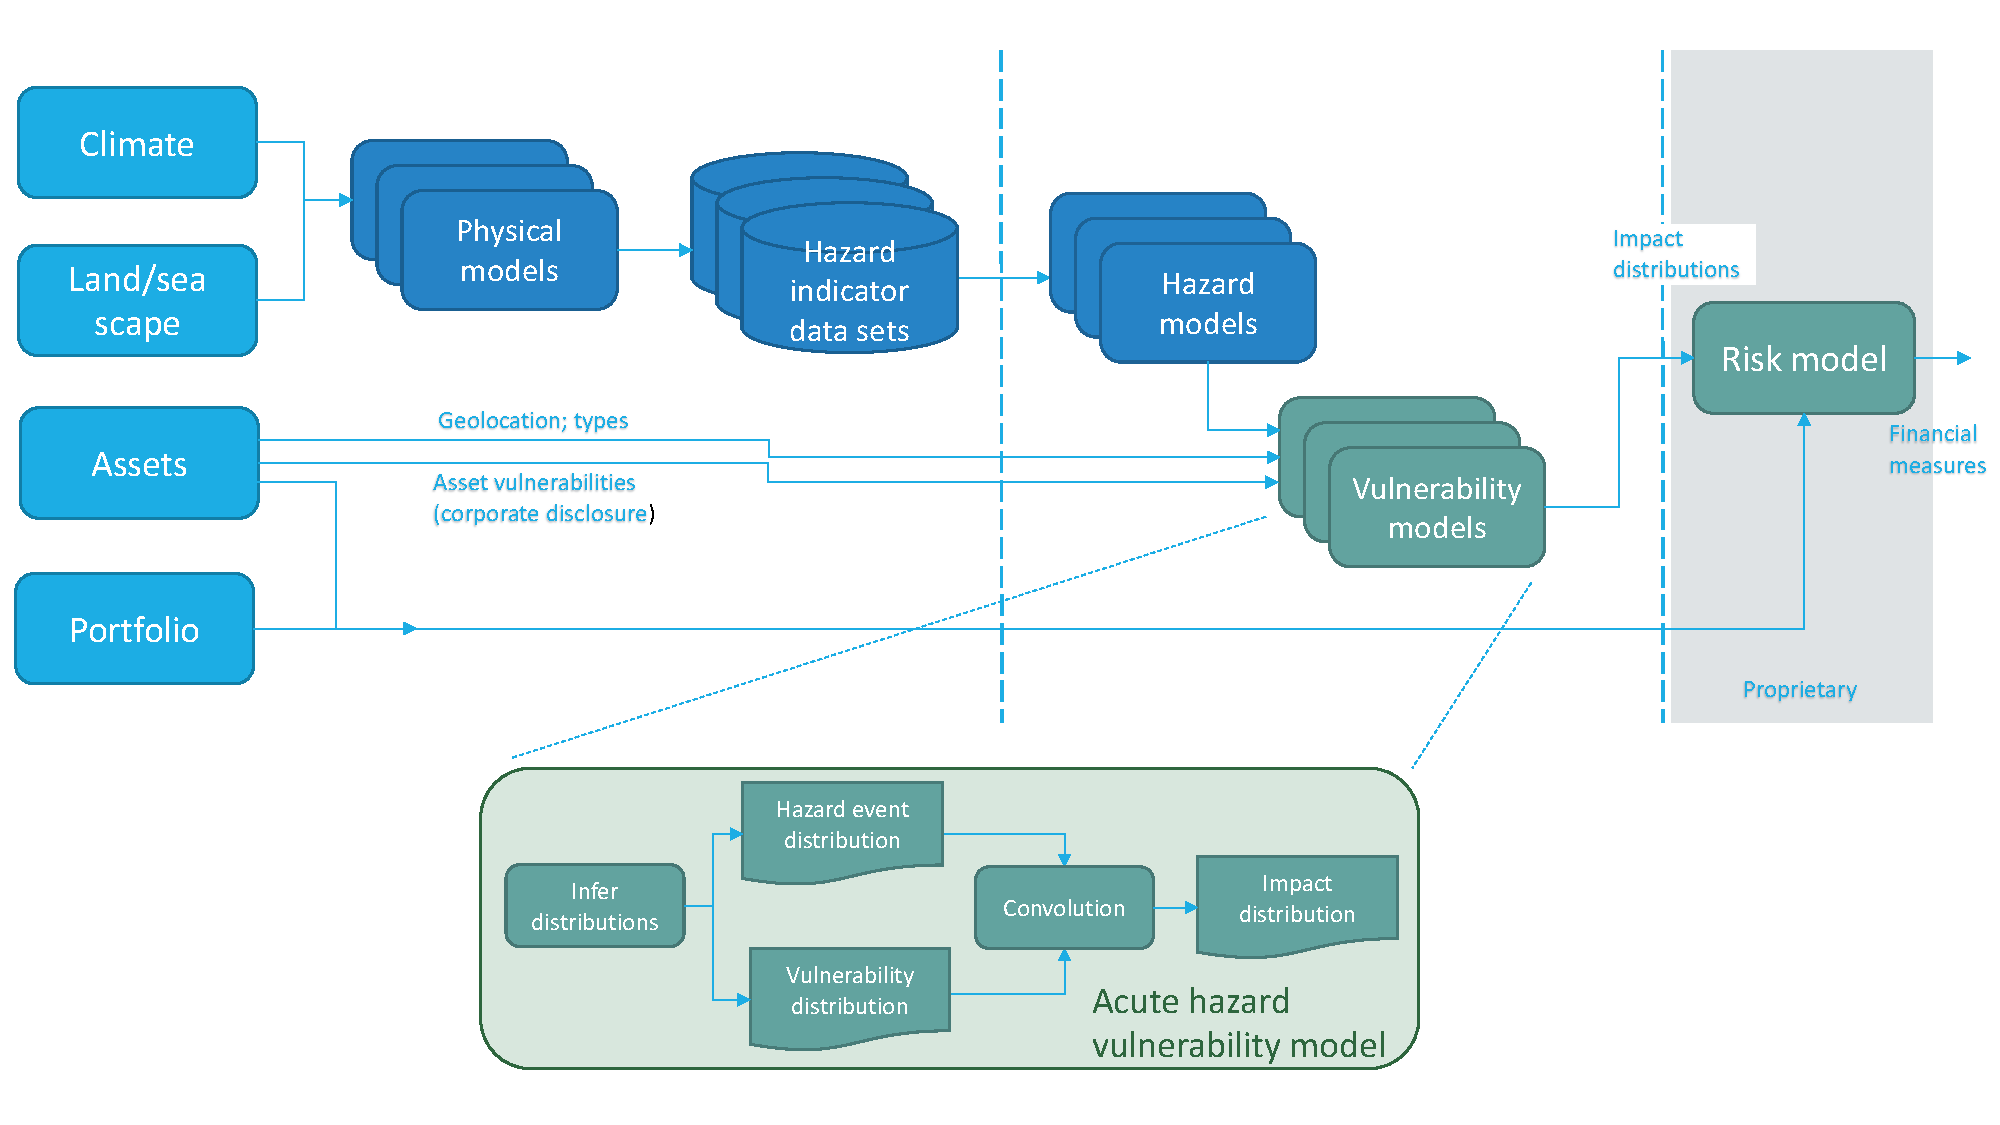
\includegraphics[clip, trim=0cm 7cm 0cm 1cm, width=1.00\textwidth]{plots/top_level_view.pdf}

    \end{framed}

    \footnotesize

    \renewcommand{\arraystretch}{1.01}

    \vspace{-3ex}

    \vspace{-0.5ex}

    \caption{\small Physical risk model components. }
    \label{Fig:top_level_view}

\end{figure}
%%%%%%%%%%%%%%%%%%%%%%%%%%%%%%%%%%%%%%%%%%%%%%%%%

\subsection{Asset impact model}
The {\it asset impact} model is used to determine how an asset is impacted by an event. The impact is a quantity from which financial loss can be inferred, but is not itself a monetary value. For example, a response might be the damage sustained to a building as a fraction of its value or the annual loss of energy output of a power station as a fraction of its annual output\footnote{A systemic change in annual output changes asset value, since this is partly determined by the expected future cash flows generated by the asset.}. In each case, a further model is required to translate the impact to a change in asset value. In principle an impact might lead to an increase or decrease in value.

Catastrophe models sometimes define a quantity `damage', and talk about `damageability'. `Damage' and `impact' are analagous quantities here but `impact' is perhaps better-suited to situations where there is, say, a decrease in output efficiency of a plant as a result of a period of higher temperatures.

Asset impact models as used in physical risk calculations may overlap with those of catastrophe models. OS-C aims to support a wide range of models, but it is desirable to identify approaches that generalize a large class of these. One such approach is adopted from Oasis \cite{OasisLMF}. The first assumption behind this is that a model should capture two important types of uncertainty, doing so by representing each by a probability distributions:
\begin{enumerate}
    \item Uncertainty as to the frequency and intensity (or severity) of events that potentially lead to a change in asset value. This is sometimes called the {\it primary uncertainty}
    \item Uncertainty as to the vulnerability of assets to events (i.e. response of assets to events of a given intensity), the {\it secondary uncertainty}
\end{enumerate}

These quantities are defined more precisely in \ref{Sec:MathematicalDescriptionOfAssetImpactModel}. Impact can be modelled using a {\it mean impact curve} (or {\it mean damage curve} in catastrophe modelling nomenclature). This is a curve relating an event intensity to an impact (e.g. a wind event with a given maximum gust speed will cause a given fractional damage to a property). In general, however, there is uncertainty as to the impact on an asset to an event of a given intensity -- in the example, the wind may cause mild or severe damage. For this reason, the vulnerability is represented rather as a two dimensional curve.

A second assumption is that the probabilities of such events may not be readily represented by distributions such as beta, gamma, beta-Bernoulli or truncated Gaussian and may be complex and multi-modal. Discrete probability distributions are therefore used in order to represent the range of possible distributions: a non-parametric approach.

\subsubsection{Mathematical description of asset impact model}
\label{Sec:MathematicalDescriptionOfAssetImpactModel}

There are $n$ intensity bins with index $i$ such that $i \in \{1, \dots, n \}$. We define $e^{(a)}_i$ to be the probability that a hazard event of type $a$ occurs with an intensity that falls in bin $i$. If $S^{(a)}$, a random variable, is the intensity of event $a$ then:

\begin{equation}
    \label{Eq:event}
    e^{(a)}_i = P \left( s^{(a, \text{lower})}_i < S^{(a)} \le s^{(a, \text{upper})}_i \right)
\end{equation}

That is, $s^{(a, \text{lower})}_i$ and $s^{(a, \text{upper})}_i$ define the range of bin $i$.

We define $v^{(a, b)}_{ij}$ to be the conditional probability that \emph{given} the occurrence of an event of type $a$ with intensity $S^{(a)}$ there is an impact (typically a damage or disruption\footnote{$d$ for `damage/disruption' is used to denote impact as $i$ is reserved for indexing}), $D^{(b)}$ in the range $d^{(a,b,\text{lower})}_j < D \le d^{(a,b,\text{upper})}_j$. The impact is of type $b$.


\begin{equation}
    \label{Eq:vulnerability}
    v^{(a, b)}_{ij} = P \left( d^{(a,b,\text{lower})}_j < D^{(b)} \le d^{(a,b,\text{upper})}_j | s^{(a, \text{lower})}_i < S^{(a)} \le s^{(a, \text{upper})}_i \right)
\end{equation}

The definition of an event type $a$ includes a time interval e.g. $a$ is the occurrence of an inundation in the locale of the asset {\it within a one year period}. $b$ is, for example, the fractional damage to the asset.

We define $d^{(a,b)}_j$ to be the marginal probability of impact $D^{(b)}$ in the range $d^{(a,b, \text{lower})}_j < D^{(b)} \le d^{(a,b,\text{upper})}_j$ occurring as a result of an event of type $a$.

\begin{equation}
    \label{Eq:impact}
    d^{(a,b)}_j = P \left( d^{(a,b,\text{lower})}_j < D^{(b)} \le d^{(a,b,\text{upper})}_j \right)
\end{equation}

From the definition of conditional probability:

\begin{equation}
    \label{Eq:model}
    d^{(a,b)}_j = \sum_{i} v^{(a,b)}_{ij} e^{(a)}_i
\end{equation}

If only the mean impact curve is available, then it is possible to create the matrix such that $v_{ij} \in \{0, 1\}$. The matrix then provides a simple mapping from intensity to impact; if the number of intensity and response bins is equal then matrix $\mathbf{v}$ is simply the identity matrix. However, note that these simplifications exclude from the model any uncertainty in the parameters\footnote{A better approach would be to estimate the standard deviation of the distributions from which the mean impact curve was calculated and to incorporate this.}.

Note that $d^{(a,b)}_j$ is identical to the {\it effective damage} distribution of Oasis and can be described as the `effective impact'. It is a marginal distribution and does not capture any correlation between events nor impacts.

%%%%%%%%%%%%%%%%%%%%%%%%%%%%%%%%%%%%%%%%%%%%%%%%%
\begin{figure}[ht]

    \begin{framed}

        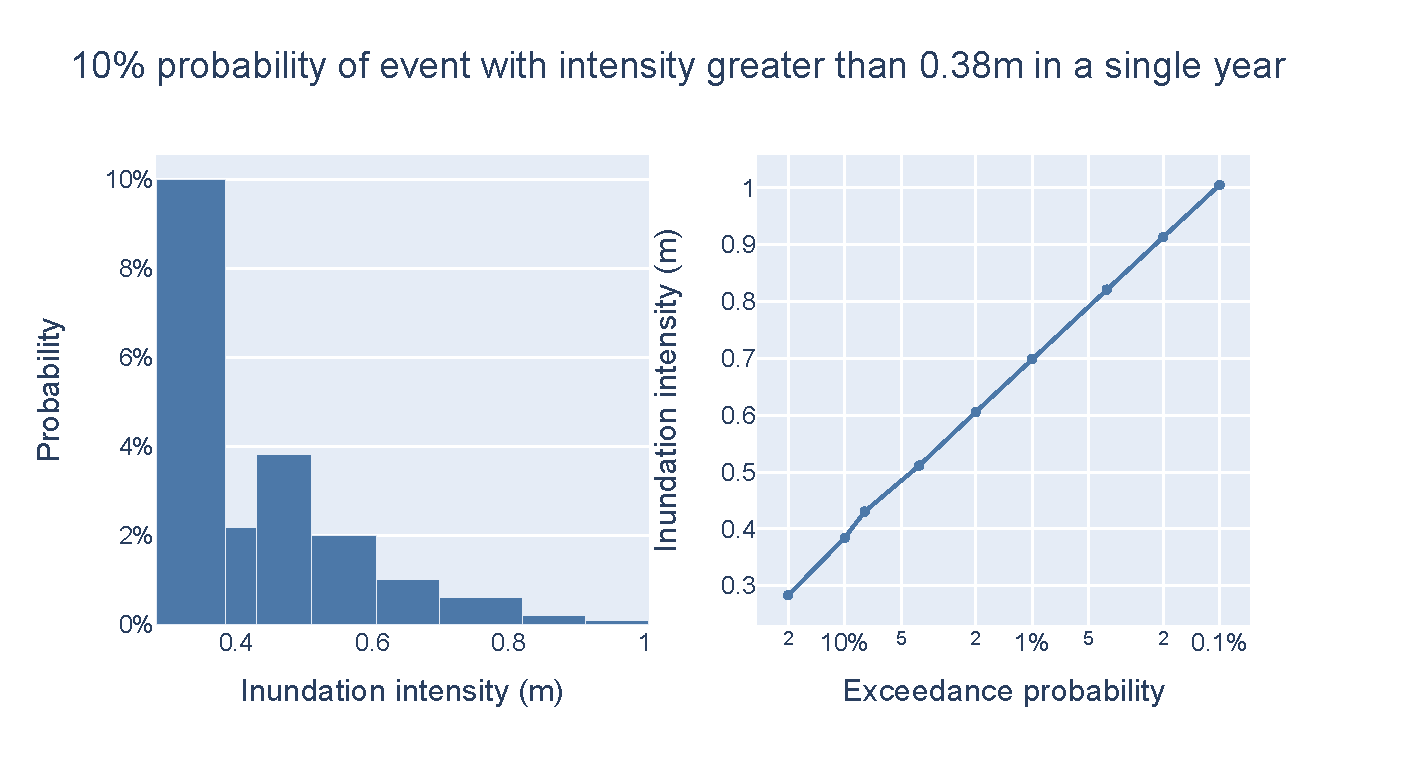
\includegraphics[width=\textwidth]{plots/fig_intensity.pdf}

    \end{framed}

    \footnotesize

    \renewcommand{\arraystretch}{1.01}

    \vspace{-3ex}

    {\justify
        The exceedance curve of event intensity at the asset location is shown on the right. The event intensity in this example is inundation depth in metres. Exceedance is a cumulative probability. As an example, the probability of an inundation event occurring within a single year of intensity 0.91m or greater is 0.002. An exceedance probability is the reciprocal of the return period; it could equivalently be said that the 0.91m intensity event occurs with a return period of 500 years.
        The exceedance curve can be converted to a histogram of probabilities. Here the $n$ bins have ranges $[s^{(a, \text{lower})}_i, s^{(a, \text{upper})}_i]$. For example, the first bin has range [0.28m, 0.38m]. The second bin has range [0.38m,    0.51m]; that is $s^{(a, \text{lower})}_2 = 0.38$m and $s^{(a, \text{upper})}_2 = 0.51$m. $e^{(a)}_2 = 0.06$.
        \par}

    \vspace{-0.5ex}

    \caption{\small Event intensity exceedance curve (right) and corresponding histogram (left).}
    \label{Fig:intensity}

\end{figure}
%%%%%%%%%%%%%%%%%%%%%%%%%%%%%%%%%%%%%%%%%%%%%%%%%

\subsubsection{Importance of secondary uncertainty}
The importance of the vulnerability matrix as opposed to mean damage curve (or vector) is emphasized above; see also \cite{Taylor:2015} for a discussion of this point. This is true not only in cases where the underlying distribution of an impact, for example a fractional damage, can be inferred from empirical data; see for example Figure~\ref{Fig:vulnerability_matrix}). This is arguably \emph{more} important where data is limited in order that approximate data can be incorporated into the model in a way that the impact of the approximations can be well-understood.

Vulnerability data may be provided by
\begin{itemize}
    \item Modelling of asset vulnerability based on asset characteristics and/or historical data
    \item 'Calibrated' vulnerabilities, for example based on realized insurance claims
\end{itemize}
Physical risk models may make use of so-called `bulk assessment' approaches for certain assets, where precise vulnerability information is not available and less precise estimates of the damage/disruption of the asset are used. The presence of such estimates in an overall model may, or may not, materially impact the accuracy of the results, but it is important that this impact can be assessed. By quantifying the uncertainty in the response estimates, a distribution of financial losses is ultimately obtained from which the model user can derive the impact of the approximation.

\paragraph{Handling epistemic uncertainty}
In forms of bulk-assessment, a common case is that insufficient information exists with which to characterize an asset. This is an example of an epistemic, as opposed to aleatory, uncertainty. The epistemic uncertainty, and its impact, can be included in the model in a relatively straight-forward way.

We extend Equation~{\ref{Eq:vulnerability}, by including a new discrete random variable, $A$, which is the type of the asset.
\begin{equation}
    \label{Eq:vulnerability}
    v^{(a, b)}_{ij} = P \left( d^{(a,b,\text{lower})}_j < D^{(b)} \le d^{(a,b,\text{upper})}_j | s^{(a, \text{lower})}_i < S^{(a)} \le s^{(a, \text{upper})}_i, A = a_1 \right)
\end{equation}


\subsubsection{Interpolation of probability distributions}
Cases arise where the event distributions and vulnerability distributions are not defined for a common set of intensity bins and interpolation is therefore required. The question then arises of how probability density is distributed within bins. The choice is model-specific and customizable, but here two common cases are described.

\begin{itemize}
    \item Probability density constant across bin: linear interpolation of cumulative probability function
    \item Probability density changes linearly across bin: quadratic interpolation of cumulative probability function
\end{itemize}

{\textcolor{red}{\emph{[Add equations and example plots here]}}}

Hazard data sets might also contain instances of `point-probabilities', for example where there is a finite probability that the intensity of an event takes a single value. These represent Dirac delta functions in the probability distribution, steps in the cumulative probability function. There is the option of retaining these as delta functions (bins of zero width), but in some cases it may be necessary to make assumptions about how these the probability might be distributed across a bin.

{\textcolor{red}{\emph{[Add equations and plot of step-CDF with interpolation; exemplify by `damage threshold']}}}

%%%%%%%%%%%%%%%%%%%%%%%%%%%%%%%%%%%%%%%%%%%%%%%%%
\begin{figure}[ht]

    \begin{framed}

        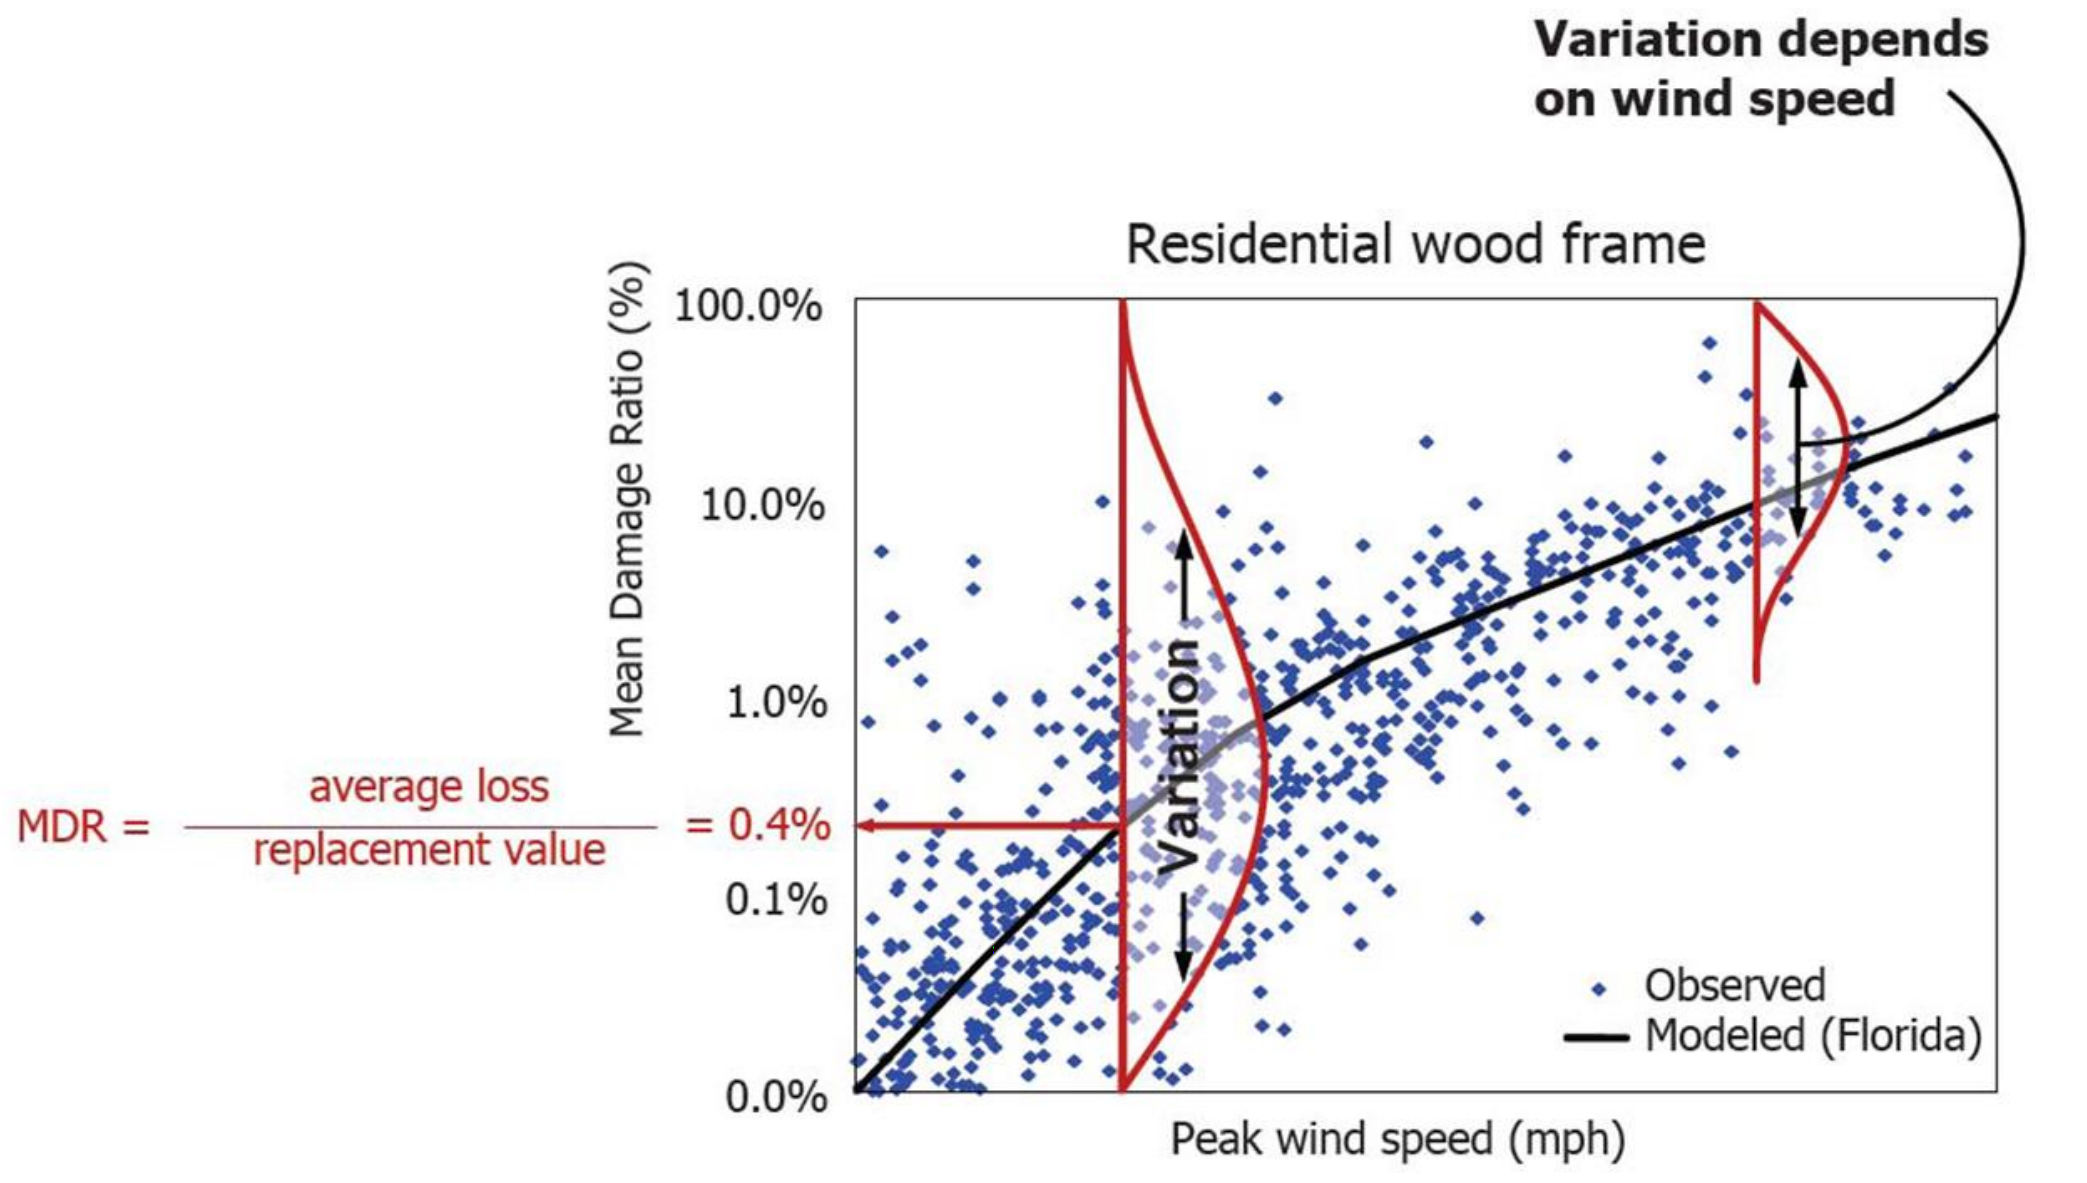
\includegraphics[width=\textwidth]{plots/vulnerability_lagace_2008.png}

    \end{framed}

    \footnotesize

    \renewcommand{\arraystretch}{1.01}

    \vspace{-3ex}

%    {\justify
%        Taken from
%        \par}

    \vspace{-0.5ex}

    \caption{\small Taken from Lagacé (2008) Catastrophe Modeling, Université Laval. Mean damage curve as an approximation to an underlying set of distributions, modelled using a vulnerability matrix. {\textcolor{red}{\emph{[To seek permission or replace e.g. with synthetic plot]}}}}
    \label{Fig:vulnerability_matrix}

\end{figure}
%%%%%%%%%%%%%%%%%%%%%%%%%%%%%%%%%%%%%%%%%%%%%%%%%




\subsection{Effective impact distribution}
$d^{(a,b)}_j$ from Equation~\ref{Eq:vulnerability} is the probability distribution of impacts of type $b$ for an asset as a result of events of type $a$. In the catastrophe models of Oasis, impacts are sampled from this distribution \cite{OasisFinancialModule}, for example samples of fractional damage, which form the basis of a Monte Carlo calculation. This is done in order to apply insurance policy terms and conditions which can be complex and non-linear.

The Monte Carlo sampling is done by constructing a cumulative probability density function, $Y_D(d)$, of impact $D$ from the effective impact distribution ($Y_D(d) = P(D \le d$)). Random numbers, $u_i$ are then sampled from a standard uniform distribution ($u_i \in [0, 1]$), from which impacts are calculated by:

\begin{equation}
    \label{Eq:sampling}
    d_i = Y^{-1}_D(u_i)
\end{equation}

In this Monte Carlo approach, samples of fractional damage can be drawn from distributions so as to be correlated or uncorrelated. For example, if the impact distributions represent damage to buildings as a result of inundation then it may be appropriate to model damage to two buildings in close proximity as being highly correlated\footnote{Catastrophe model practitioners might point out that presence or absence of kerb stones and availability of sand bags are highly significant so any such assumption is prone to error}. If the buildings are far apart (say in different countries) then the correlation is likely to be close to zero.

\subsubsection{Full Monte Carlo calculation}
A more sophisticated correlation model might try to capture correlation of events and of vulnerabilities. Such models would typically need to first sample from the distribution of event intensity and then from the vulnerability distribution. This is more computationally expensive than the approach of deriving an effective impact distribution. Such a `full Monte Carlo' approach might prove to be relevant for some models as it is a highly flexible approach.


\subsection{Aggregation of impacts}
For impacts of the same type, $b$, arising from different events, it is assumed that the impacts are additive, up to a ceiling value\footnote{this approximation is only strictly valid for sufficiently small impacts; consider the contrived example of 0.8 fractional damage that occurs from both flood and high wind in the same year.}. If the annual impacts from events with index 1 and 2 are represented by random variables, $Y^{(1,b)}$, $Y^{(2,b)}$ then $Y^{(\text{tot}, b)} = Y^{(1,b)} + Y^{(2,b)}$.

If the random variables are uncorrelated, then the aggregated effective impact distribution is given by the convolution:

\begin{equation}
    \label{Eq:sampling}
    y^{(\text{tot}, b)}(r) = \int^{\infty}_{-\infty} y^{(1, b)}(t) y^{(2, b)}(r - t) dt
\end{equation}

{\textcolor{red}{\emph{[Add version with discrete binned data.]}}}

\subsection{Financial loss model}
Several financial measures are of interest.

\begin{enumerate}
    \item Annual Exceedance Probability (AEP): the probability that in a given year the aggregated losses of a portfolio will exceed a certain value
    \item Valuation Adjustment: an adjustment to the present value of an asset to reflect the expected loss
\end{enumerate}

The first of these typically requires less data in its calculation. This is a cumulative probability distribution of losses from which the average annual loss (AAL) can be inferred, but also the range of losses in a given confidence interval. This interval is driven by the primary and secondary uncertainties above.

With additional modelling steps, credit risk measures can also be derived.

\subsubsection{Structural models of credit risk}
Changes in asset value can be used to model changes in the credit quality of market participants. Financial risk modules for physical risk may then use distributions of asset value changes in order to model changes of credit quality over time as a result of climate change, for example estimates of default probability and loss given default.

The intention of this section is not to specify any particular model, but rather to give a brief introduction. Particularly of interest is the question of what inputs credit risk models require.

For medium and large cap firms, a credit default event typically occurs when a firm is not able to meet its debt servicing obligations. Under an important class of credit risk models called `structural models', it is assumed that a default event occurs for a firm when its assets are sufficiently low compared to its liabilities.

A number of different structural models exist which make various assumptions about how a firm's assets change over time, how its capital is structured and the nature of its debt.

The earliest structural model was described by Merton in 1974 \cite{Merton:1974} based on an extremely simple debt structure. Black and Cox \cite{BlackCox:1976} introduced an important refinement to the Merton model in 1976. Practical implementations were subsequently created as a result of this foundational work. A notable one of these is the `KMV' model, named after Kealhofer, McQuown and Vasiek, now owned by Moody's Investors Service, Inc.

Use of such credit models, may provide a mechanism for incorporation of physical risk into financial institutions existing risk models\cite{KenyonEtAl:2021}.

\subsection{Uncertainties in the calculation}

\subsection{Model limitations}

\begin{enumerate}
    \item Spatial correlation of events: to what extent possible without MC calculation; to what extent is provided / can be inferred from data sets
    \item Correlation of vulnerability
    \item Data availability
\end{enumerate}


\subsubsection{Data availability}
Issues related to data availability and relevance are still one of the main limitations of physical risks assessments. If past and future climate data are becoming increasingly available through open-sources portals and tools (e.g. Copernicus, WRI Aqueduct), their availability and their reliability varies widely according to the climate hazard of interest, the region and the modelling process. If the availability of climate data is improving, open-source, asset-level information (required to estimate the exposure of an asset to a give climate hazard) is still seldom available. Such data include the location of assets, their link with owning companies and more generally any damages records that could be used to quantify the response of an asset (or of a type of asset) to a given climate event. Newly-published datasets have been recently released for some sectors but their exhaustiveness remains to be verified. Moreover, many industrial sectors are not covered, thus limiting the application of physical risks methodologies to a diversified portfolio.
Finally, building and applying the correlation between hazard and damage (or impact), as described in section 2.2, requires common distribution between historical events, historical damages and future climate events. In a changing climate, assets and activities will be impacted by more intense events that will not have been experienced either in a given region of the world or even on the
whole globe, leading to a potentially large mismatch between historical and future distributions of events. The interpolation of the damage curve, as described in section 2.2.3, might lead to very high uncertainties that need to be taken into account when interpreting the data.




\clearpage
%%%%%%%%%%%%%%%%%%%%%%%%%%%%%%%%%%%%%%%%%%%%%%%%%%%%%%%%%%%%%%%
\bibliography{Physical Risk Methodology Bibliography}
%%%%%%%%%%%%%%%%%%%%%%%%%%%%%%%%%%%%%%%%%%%%%%%%%%%%%%%%%%%%%%%

%\bibliographystyle{plain}
\bibliographystyle{acm}
%\bibliographystyle{agsm}


\end{document}
